\documentclass[11ppt]{article}

\usepackage{hyperref}
\usepackage{geometry}
\usepackage{graphicx}

\geometry{
  margin=0.5in
}

% Custom section fonts
\usepackage{sectsty}
\usepackage[document]{ragged2e}
\usepackage{xcolor}

\begin{document}
{\rmfamily\mdseries\Large Assignment Part 1 \hfill Buridi Sree Aditya - 15CS30008}\\
\hrulefill \\
\vspace{3mm}
\textit{\underline{SUB PART 1 - Zipf's law verification}}\\
\vspace{3mm}
From Zipf's law : $ f\propto \frac{1}{r}$\\
$ f*r = constant $ \\
$ \log f + \log r = constant $ \\
$ \log f = -\log r + constant $ \\


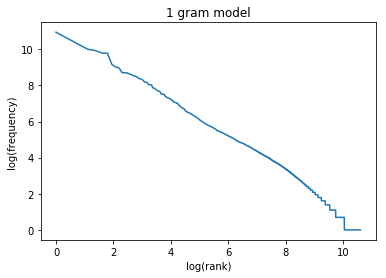
\includegraphics[scale=0.6]{unigram}
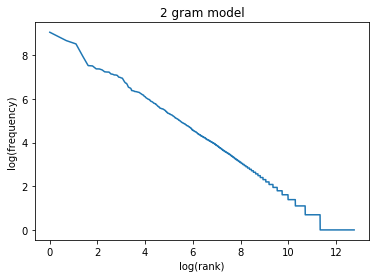
\includegraphics[scale=0.6]{bigram}

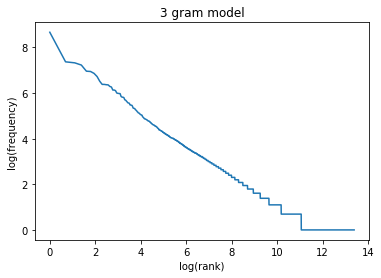
\includegraphics[scale=0.6]{trigram}

\vspace{3mm}
\textit{\underline{SUB PART 2 - Top 10 N-grams}}\\
\vspace{3mm}
\textit{Top 10 unigrams:} \\ \vspace{1mm}
(('the',), 56448) \\
(('of',), 31276) \\
(('and',), 22092) \\
(('to',), 20341) \\
(('a',), 17780) \\
(('in',), 17705) \\
(('is',), 9474) \\
(('that',), 8240) \\
(('for',), 7788) \\
(('it',), 6051) \\
\vspace{2mm}
\textit{Top 10 bigrams:} \\ \vspace{1mm}
(('of', 'the'), 8508) \\
(('\textless s\textgreater', 'the'), 5798) \\
(('in', 'the'), 4985) \\
(('to', 'the'), 2819) \\
(('and', 'the'), 1848) \\
(('on', 'the'), 1821) \\
(('for', 'the'), 1591) \\
(('\textless s\textgreater', 'in'), 1585) \\
(('\textless s\textgreater', 'it'), 1516) \\
(('it', 'is'), 1390) \\
\vspace{2mm}
\textit{Top 10 trigrams:} \\ \vspace{1mm}
(('\textless s\textgreater', '\textless s\textgreater', 'the'), 5798) \\
(('\textless s\textgreater', '\textless s\textgreater', 'in'), 1585) \\
(('\textless s\textgreater', '\textless s\textgreater', 'it'), 1516) \\
(('\textless s\textgreater', '\textless s\textgreater', 'he'), 1377) \\
(('\textless s\textgreater', '\textless s\textgreater', 'this'), 1052) \\
(('\textless s\textgreater', '\textless s\textgreater', 'but'), 1038) \\
(('\textless s\textgreater', '\textless s\textgreater', 'a'), 955) \\
(('\textless s\textgreater', '\textless s\textgreater', 'and'), 831) \\
(('\textless s\textgreater', '\textless s\textgreater', 'i'), 675) \\
(('\textless s\textgreater', '\textless s\textgreater', 'they'), 590) \\
\vspace{3mm}
\textit{\underline{SUB PART 3 - Log Likelihood and Perplexity Score over testcases}}\\
\vspace{3mm}
\textit{Below models are run on these test examples :}\\  'he', 'lived', 'a', 'good', 'life',\\ 'the', 'man', 'was', 'happy',\\ 'the', 'person', 'was', 'good',\\ 'the', 'girl', 'was', 'sad',\\ 'he', 'won', 'the', 'war'\\
\vspace{2mm}
\textit{Loglikelihood for unigram model:} \\ \vspace{1mm}  [-32.83424838102342, -24.091989655768156, -23.4166871259785, -27.32603162480786, -24.734905768951318]  \\ \vspace{2mm}
\textit{Loglikelihood for bigram model:} \\ \vspace{1mm}  [-26.86317000488739, -22.339591199881653, -24.838201556634292, -inf, -21.15431998899194]  \\ \vspace{2mm}
\textit{Loglikelihood for trigram model:} \\ \vspace{1mm}  [-inf, -inf, -inf, -inf, -15.995702002744252]  \\ \vspace{2mm}
\textit{Perplexity for unigram model:} \\ \vspace{1mm}  [0.0014062204912880043, 0.002422397773280329, 0.0028679098737995246, 0.0010792295131443134, 0.0020627268823580876]  \\ \vspace{2mm}
\textit{Perplexity for bigram model:} \\ \vspace{1mm}  [0.004641888454787715, 0.003754133422712128, 0.0020101410421309316, inf, 0.005048924658664008]  \\ \vspace{2mm}
\textit{Perplexity for trigram model:} \\ \vspace{1mm}  [inf, inf, inf, inf, 0.01833532960709163]  \\ 
\vspace{4mm}

{\rmfamily\mdseries\Large Assignment Part 2 - Laplace Smoothing}\\
\hrulefill \\
\vspace{3mm}
\textit{Below models are run on these test examples :}\\  'he', 'lived', 'a', 'good', 'life',\\ 'the', 'man', 'was', 'happy',\\ 'the', 'person', 'was', 'good',\\ 'the', 'girl', 'was', 'sad',\\ 'he', 'won', 'the', 'war'\\
\vspace{2mm}
\textit{Inference: }Performance degrades with increasing Laplace constant.\\ \vspace{2mm}

\textit{\textbf{Laplace Constant : 0.0001 }}\\ \vspace{2mm}
\textit{Loglikelihood for unigram model:} \\ \vspace{1mm}  [-32.834746262759, -24.092387694914404, -23.417086174791734, -27.326424651312145, -24.73530387061002]  \\ \vspace{2mm}
\textit{Loglikelihood for bigram model:} \\ \vspace{1mm}  [-26.95176691962215, -22.4215321021218, -24.8783195499466, -35.28121184282719, -21.2340140486702]  \\ \vspace{2mm}
\textit{Loglikelihood for trigram model:} \\ \vspace{1mm}  [-48.056460667126736, -34.873904683648725, -35.024301836829885, -36.82021816036394, -17.549621990505962]  \\ \vspace{2mm}
\textit{Perplexity for unigram model:} \\ \vspace{1mm}  [0.001406080471959667, 0.0024221567329880747, 0.0028676237790625806, 0.001079123476903062, 0.0020625215988253906]  \\ \vspace{2mm}
\textit{Perplexity for bigram model:} \\ \vspace{1mm}  [0.004560361492511085, 0.0036780115021154158, 0.0019900810996430875, 0.00014770360506426058, 0.0049493277873057994]  \\ \vspace{2mm}
\textit{Perplexity for trigram model:} \\ \vspace{1mm}  [6.696823647655817e-05, 0.00016353620237026233, 0.00015750151838466952, 0.00010052998265414904, 0.012432944715356702]  \\ \vspace{2mm}
\textit{\textbf{Laplace Constant : 0.001 }}\\ \vspace{2mm}
\textit{Loglikelihood for unigram model:} \\ \vspace{1mm}  [-32.83922495016433, -24.095968248693975, -23.420675815456175, -27.32996009277662, -24.738884986977126]  \\ \vspace{2mm}
\textit{Loglikelihood for bigram model:} \\ \vspace{1mm}  [-27.57949052214715, -22.982879841217674, -25.198449120216807, -34.36277391875188, -21.798876178603518]  \\ \vspace{2mm}
\textit{Loglikelihood for trigram model:} \\ \vspace{1mm}  [-47.48395016865736, -35.257292068140536, -35.89132398864079, -39.83687900149157, -21.537488157082798]  \\ \vspace{2mm}
\textit{Perplexity for unigram model:} \\ \vspace{1mm}  [0.0014048215568924153, 0.0024199895374915326, 0.002865051498698575, 0.0010781701038180861, 0.0020606758926959615]  \\ \vspace{2mm}
\textit{Perplexity for bigram model:} \\ \vspace{1mm}  [0.004022313258438062, 0.003196432418563176, 0.0018370168870582356, 0.0001858271755895745, 0.0042975119301188955]  \\ \vspace{2mm}
\textit{Perplexity for trigram model:} \\ \vspace{1mm}  [7.509248778199658e-05, 0.0001485895104949571, 0.0001268086884816192, 4.728961936127632e-05, 0.004587720326082994]  \\ \vspace{2mm}
\textit{\textbf{Laplace Constant : 0.01 }}\\ \vspace{2mm}
\textit{Loglikelihood for unigram model:} \\ \vspace{1mm}  [-32.88379072368735, -24.13159690954856, -23.456395333476458, -27.365137775214055, -24.77451927127337]  \\ \vspace{2mm}
\textit{Loglikelihood for bigram model:} \\ \vspace{1mm}  [-30.223692391114643, -25.06582382115037, -26.910112293042992, -35.482481560924576, -24.060599831541595]  \\ \vspace{2mm}
\textit{Loglikelihood for trigram model:} \\ \vspace{1mm}  [-49.88941160326865, -38.58944042024911, -39.57718998337484, -44.21534495761073, -29.066705800378298]  \\ \vspace{2mm}
\textit{Perplexity for unigram model:} \\ \vspace{1mm}  [0.0013923558021514107, 0.0023985300045472574, 0.002839580828306346, 0.001068729794307094, 0.0020423997431042017]  \\ \vspace{2mm}
\textit{Perplexity for bigram model:} \\ \vspace{1mm}  [0.002370300643168069, 0.0018989466234006487, 0.0011974894086604388, 0.00014045542346669595, 0.0024414822175878965]  \\ \vspace{2mm}
\textit{Perplexity for trigram model:} \\ \vspace{1mm}  [4.641525781091414e-05, 6.459586845265215e-05, 5.046162074610827e-05, 1.5826319077130773e-05, 0.000698429405594697]  \\ \vspace{2mm}
\textit{\textbf{Laplace Constant : 0.1 }}\\ \vspace{2mm}
\textit{Loglikelihood for unigram model:} \\ \vspace{1mm}  [-33.30870752682203, -24.471291120260428, -23.796996949108927, -27.700336616381716, -25.114269473477272]  \\ \vspace{2mm}
\textit{Loglikelihood for bigram model:} \\ \vspace{1mm}  [-36.21855054341226, -29.317741128330834, -31.065751514978366, -38.07733662405666, -28.62157925834711]  \\ \vspace{2mm}
\textit{Loglikelihood for trigram model:} \\ \vspace{1mm}  [-55.12612222826344, -43.5270098579958, -44.52756214051961, -49.12329885182458, -38.96406984927926]  \\ \vspace{2mm}
\textit{Perplexity for unigram model:} \\ \vspace{1mm}  [0.0012789171887368912, 0.0022032476996306136, 0.0026077976208990715, 0.0009828204063062555, 0.0018760864106040253]  \\ \vspace{2mm}
\textit{Perplexity for bigram model:} \\ \vspace{1mm}  [0.0007146553862849615, 0.0006559439058294111, 0.0004237199235148975, 7.341853336802272e-05, 0.0007806412859571138]  \\ \vspace{2mm}
\textit{Perplexity for trigram model:} \\ \vspace{1mm}  [1.6285678668446664e-05, 1.8798143095943744e-05, 1.4637987347728277e-05, 4.639867663379853e-06, 5.882065658300917e-05]  \\ \vspace{2mm}
\textit{\textbf{Laplace Constant : 1 }}\\ \vspace{2mm}
\textit{Loglikelihood for unigram model:} \\ \vspace{1mm}  [-36.27920152752997, -26.845328323359098, -26.179993069333047, -30.030805343716295, -27.488842731794616]  \\ \vspace{2mm}
\textit{Loglikelihood for bigram model:} \\ \vspace{1mm}  [-44.84569996153263, -35.98692274903626, -37.36846750466741, -42.033583729302975, -35.46543785693498]  \\ \vspace{2mm}
\textit{Loglikelihood for trigram model:} \\ \vspace{1mm}  [-61.50885898889724, -49.948556485876885, -50.47066210038483, -54.15842061297218, -48.94623303501051]  \\ \vspace{2mm}
\textit{Perplexity for unigram model:} \\ \vspace{1mm}  [0.0007060388416337418, 0.001217041846214115, 0.0014372865729122277, 0.0005488412414677287, 0.0010361838567876675]  \\ \vspace{2mm}
\textit{Perplexity for bigram model:} \\ \vspace{1mm}  [0.00012727760482017606, 0.00012381392957789048, 8.7653687550773e-05, 2.7306223019279004e-05, 0.00014105517046341436]  \\ \vspace{2mm}
\textit{Perplexity for trigram model:} \\ \vspace{1mm}  [4.5436868327046525e-06, 3.7748907296540824e-06, 3.3129698834770587e-06, 1.317723207737269e-06, 4.849871933862789e-06]  \\ 
\vspace{4mm}


{\rmfamily\mdseries\Large Assignment Part 3 - Good-Turing Method}\\
\hrulefill \\
\vspace{3mm}
\textit{Below models are run on these test examples :}\\  'he', 'lived', 'a', 'good', 'life',\\ 'the', 'man', 'was', 'happy',\\ 'the', 'person', 'was', 'good',\\ 'the', 'girl', 'was', 'sad',\\ 'he', 'won', 'the', 'war'\\
\vspace{2mm}
\textit{Inference: }\\
Naive implementation of this method fails mainly because of 2 ways:\\
1. Cases where $n_{r+1} = 0$\\
2. Case where $n_{r+1} = 0$ because of r being the highest frequency.\\
\vspace{2mm}
\textit{Loglikelihood for unigram model:} \\ \vspace{1mm}  [-32.83424838102342, -24.091989655768156, -23.4166871259785, -27.32603162480786, -24.734905768951318]  \\ \vspace{2mm}
\textit{Loglikelihood for bigram model:} \\ \vspace{1mm}  [-inf, -inf, -inf, -inf, -inf]  \\ \vspace{2mm}
\textit{Loglikelihood for trigram model:} \\ \vspace{1mm}  [-84.30398062496148, -50.35520597619277, -51.450965195878474, -56.213139130676225, 13.656538272857798]  \\ \vspace{2mm}
\textit{Perplexity for unigram model:} \\ \vspace{1mm}  [0.0014062204912880043, 0.002422397773280329, 0.0028679098737995246, 0.0010792295131443134, 0.0020627268823580876]  \\ \vspace{2mm}
\textit{Perplexity for bigram model:} \\ \vspace{1mm}  [inf, inf, inf, inf, inf]  \\ \vspace{2mm}
\textit{Perplexity for trigram model:} \\ \vspace{1mm}  [4.758272199069103e-08, 3.409988994654197e-06, 2.592880082845027e-06, 7.883806678796675e-07, 30.390637020150237]  \\ 
\vspace{4mm}
{\rmfamily\mdseries\Large Assignment Part 4 - Interpolation Method}\\
\hrulefill \\
\vspace{3mm}
\textit{Below models are run on these test examples :} \\ 
\ ['he', 'lived', 'a', 'good', 'life'] \\
\ ['the', 'man', 'was', 'happy'] \\
\ ['the', 'person', 'was', 'good'] \\
\ ['the', 'girl', 'was', 'sad'] \\
\ ['he', 'won', 'the', 'war'] \\
\vspace{2mm}

\textit{Inference: }The performance increases with increasing $\lambda$ value.\\
\textit{Inference: } $\lambda$ for bigram interpolation; $\lambda_{1}$ and $\lambda_{2}$ for trigram interpolation.\\
\vspace{2mm}
\textit{\textbf{Using Interpolation smoothing with $\lambda = $ 0.2 $\lambda_{1} = $ 0.2 $\lambda_{2} = $ 0.2}} \\ \vspace{2mm}
Loglikelihood for bigram model: \\ \vspace{1mm}  [-32.66246276441453, -26.719690688001492, -27.40283499806891, -31.35563915688864, -26.34077593024058]  \\ \vspace{2mm}
Loglikelihood for trigram model: \\ \vspace{1mm}  [-32.5385828001288, -27.343571554618293, -27.430526465475456, -32.10895968229792, -22.62987957833191]  \\ \vspace{2mm}
Perplexity for bigram model: \\ \vspace{1mm}  [0.0014553737290567707, 0.001255875083115597, 0.0010587050702298892, 0.00039409845692069074, 0.001380659517754312]  \\ \vspace{2mm}
Perplexity for trigram model: \\ \vspace{1mm}  [0.0014918824606549154, 0.0010745074712685315, 0.001051401107345643, 0.0003264479889949162, 0.00349133918903733]  \\ \vspace{2mm}
\textit{\textbf{Using Interpolation smoothing with $\lambda = $ 0.5 $\lambda_{1} = $ 0.3 $\lambda_{2} = $ 0.3}} \\ \vspace{2mm}
Loglikelihood for bigram model: \\ \vspace{1mm}  [-29.534955832872953, -24.49074549396976, -26.05971719767102, -30.166311778821427, -23.681408966578573]  \\ \vspace{2mm}
Loglikelihood for trigram model: \\ \vspace{1mm}  [-30.688418095326107, -25.75476772679707, -26.59521806071914, -31.172438283723096, -20.573328581211484]  \\ \vspace{2mm}
Perplexity for bigram model: \\ \vspace{1mm}  [0.002720359695092117, 0.002192558014811939, 0.0014811606146854987, 0.0005305597669526547, 0.0026842545041897373]  \\ \vspace{2mm}
Perplexity for trigram model: \\ \vspace{1mm}  [0.0021599210280007055, 0.0015984962559419142, 0.0012955700143163684, 0.00041256797786982604, 0.005838203523509511]  \\ \vspace{2mm}
\textit{\textbf{Using Interpolation smoothing with $\lambda = $ 0.8 $\lambda_{1} = $ 0.5 $\lambda_{2} = $ 0.5}} \\ \vspace{2mm}
Loglikelihood for bigram model: \\ \vspace{1mm}  [-27.742016099604488, -23.07769266612461, -25.251662024964457, -30.023842061623544, -22.012408138365345]  \\ \vspace{2mm}
Loglikelihood for trigram model: \\ \vspace{1mm}  [-28.474571723720764, -23.538020160919725, -25.811653927371488, -inf, -17.845886921150193]  \\ \vspace{2mm}
Perplexity for bigram model: \\ \vspace{1mm}  [0.003893669616337511, 0.0031215576138428095, 0.0018127404712529286, 0.0005497975076672671, 0.004074113774500785]  \\ \vspace{2mm}
Perplexity for trigram model: \\ \vspace{1mm}  [0.0033630252275713628, 0.0027822229730231503, 0.001575924047619089, inf, 0.011545359123063854]  \\ \vspace{2mm}

\end{document}